\PassOptionsToPackage{unicode=true}{hyperref} % options for packages loaded elsewhere
\PassOptionsToPackage{hyphens}{url}
%
\documentclass[]{article}
\usepackage{lmodern}
\usepackage{amssymb,amsmath}
\usepackage{ifxetex,ifluatex}
\usepackage{fixltx2e} % provides \textsubscript
\ifnum 0\ifxetex 1\fi\ifluatex 1\fi=0 % if pdftex
  \usepackage[T1]{fontenc}
  \usepackage[utf8]{inputenc}
  \usepackage{textcomp} % provides euro and other symbols
\else % if luatex or xelatex
  \usepackage{unicode-math}
  \defaultfontfeatures{Ligatures=TeX,Scale=MatchLowercase}
\fi
% use upquote if available, for straight quotes in verbatim environments
\IfFileExists{upquote.sty}{\usepackage{upquote}}{}
% use microtype if available
\IfFileExists{microtype.sty}{%
\usepackage[]{microtype}
\UseMicrotypeSet[protrusion]{basicmath} % disable protrusion for tt fonts
}{}
\IfFileExists{parskip.sty}{%
\usepackage{parskip}
}{% else
\setlength{\parindent}{0pt}
\setlength{\parskip}{6pt plus 2pt minus 1pt}
}
\usepackage{hyperref}
\hypersetup{
            pdftitle={PRA2 - Tipología y ciclo de vida de dato},
            pdfborder={0 0 0},
            breaklinks=true}
\urlstyle{same}  % don't use monospace font for urls
\usepackage[margin=1in]{geometry}
\usepackage{color}
\usepackage{fancyvrb}
\newcommand{\VerbBar}{|}
\newcommand{\VERB}{\Verb[commandchars=\\\{\}]}
\DefineVerbatimEnvironment{Highlighting}{Verbatim}{commandchars=\\\{\}}
% Add ',fontsize=\small' for more characters per line
\usepackage{framed}
\definecolor{shadecolor}{RGB}{248,248,248}
\newenvironment{Shaded}{\begin{snugshade}}{\end{snugshade}}
\newcommand{\AlertTok}[1]{\textcolor[rgb]{0.94,0.16,0.16}{#1}}
\newcommand{\AnnotationTok}[1]{\textcolor[rgb]{0.56,0.35,0.01}{\textbf{\textit{#1}}}}
\newcommand{\AttributeTok}[1]{\textcolor[rgb]{0.77,0.63,0.00}{#1}}
\newcommand{\BaseNTok}[1]{\textcolor[rgb]{0.00,0.00,0.81}{#1}}
\newcommand{\BuiltInTok}[1]{#1}
\newcommand{\CharTok}[1]{\textcolor[rgb]{0.31,0.60,0.02}{#1}}
\newcommand{\CommentTok}[1]{\textcolor[rgb]{0.56,0.35,0.01}{\textit{#1}}}
\newcommand{\CommentVarTok}[1]{\textcolor[rgb]{0.56,0.35,0.01}{\textbf{\textit{#1}}}}
\newcommand{\ConstantTok}[1]{\textcolor[rgb]{0.00,0.00,0.00}{#1}}
\newcommand{\ControlFlowTok}[1]{\textcolor[rgb]{0.13,0.29,0.53}{\textbf{#1}}}
\newcommand{\DataTypeTok}[1]{\textcolor[rgb]{0.13,0.29,0.53}{#1}}
\newcommand{\DecValTok}[1]{\textcolor[rgb]{0.00,0.00,0.81}{#1}}
\newcommand{\DocumentationTok}[1]{\textcolor[rgb]{0.56,0.35,0.01}{\textbf{\textit{#1}}}}
\newcommand{\ErrorTok}[1]{\textcolor[rgb]{0.64,0.00,0.00}{\textbf{#1}}}
\newcommand{\ExtensionTok}[1]{#1}
\newcommand{\FloatTok}[1]{\textcolor[rgb]{0.00,0.00,0.81}{#1}}
\newcommand{\FunctionTok}[1]{\textcolor[rgb]{0.00,0.00,0.00}{#1}}
\newcommand{\ImportTok}[1]{#1}
\newcommand{\InformationTok}[1]{\textcolor[rgb]{0.56,0.35,0.01}{\textbf{\textit{#1}}}}
\newcommand{\KeywordTok}[1]{\textcolor[rgb]{0.13,0.29,0.53}{\textbf{#1}}}
\newcommand{\NormalTok}[1]{#1}
\newcommand{\OperatorTok}[1]{\textcolor[rgb]{0.81,0.36,0.00}{\textbf{#1}}}
\newcommand{\OtherTok}[1]{\textcolor[rgb]{0.56,0.35,0.01}{#1}}
\newcommand{\PreprocessorTok}[1]{\textcolor[rgb]{0.56,0.35,0.01}{\textit{#1}}}
\newcommand{\RegionMarkerTok}[1]{#1}
\newcommand{\SpecialCharTok}[1]{\textcolor[rgb]{0.00,0.00,0.00}{#1}}
\newcommand{\SpecialStringTok}[1]{\textcolor[rgb]{0.31,0.60,0.02}{#1}}
\newcommand{\StringTok}[1]{\textcolor[rgb]{0.31,0.60,0.02}{#1}}
\newcommand{\VariableTok}[1]{\textcolor[rgb]{0.00,0.00,0.00}{#1}}
\newcommand{\VerbatimStringTok}[1]{\textcolor[rgb]{0.31,0.60,0.02}{#1}}
\newcommand{\WarningTok}[1]{\textcolor[rgb]{0.56,0.35,0.01}{\textbf{\textit{#1}}}}
\usepackage{graphicx,grffile}
\makeatletter
\def\maxwidth{\ifdim\Gin@nat@width>\linewidth\linewidth\else\Gin@nat@width\fi}
\def\maxheight{\ifdim\Gin@nat@height>\textheight\textheight\else\Gin@nat@height\fi}
\makeatother
% Scale images if necessary, so that they will not overflow the page
% margins by default, and it is still possible to overwrite the defaults
% using explicit options in \includegraphics[width, height, ...]{}
\setkeys{Gin}{width=\maxwidth,height=\maxheight,keepaspectratio}
\setlength{\emergencystretch}{3em}  % prevent overfull lines
\providecommand{\tightlist}{%
  \setlength{\itemsep}{0pt}\setlength{\parskip}{0pt}}
\setcounter{secnumdepth}{0}
% Redefines (sub)paragraphs to behave more like sections
\ifx\paragraph\undefined\else
\let\oldparagraph\paragraph
\renewcommand{\paragraph}[1]{\oldparagraph{#1}\mbox{}}
\fi
\ifx\subparagraph\undefined\else
\let\oldsubparagraph\subparagraph
\renewcommand{\subparagraph}[1]{\oldsubparagraph{#1}\mbox{}}
\fi

% set default figure placement to htbp
\makeatletter
\def\fps@figure{htbp}
\makeatother


\title{PRA2 - Tipología y ciclo de vida de dato}
\author{}
\date{\vspace{-2.5em}}

\begin{document}
\maketitle

\emph{Alumnos: Omar Mendo Mesa y Guzmán Gómez Pérez }

\hypertarget{uxedndice}{%
\subsection{Índice}\label{uxedndice}}

\begin{enumerate}
\def\labelenumi{\arabic{enumi}.}
\item
  Descripción del dataset. ¿Por qué es importante y qué
  pregunta/problema pretende responder?
\item
  Integración y selección de los datos de interés a analizar.
\item
  Limpieza de los datos.
\end{enumerate}

3.1. ¿Los datos contienen ceros o elementos vacíos? ¿Cómo gestionarías
cada uno de estos casos?

3.2. Identificación y tratamiento de valores extremos.

\begin{enumerate}
\def\labelenumi{\arabic{enumi}.}
\setcounter{enumi}{3}
\tightlist
\item
  Análisis de los datos.
\end{enumerate}

4.1. Selección de los grupos de datos que se quieren analizar/comparar
(planificación de los análisis a aplicar).

4.2. Comprobación de la normalidad y homogeneidad de la varianza.

4.3. Aplicación de pruebas estadísticas para comparar los grupos de
datos. En función de los datos y el objetivo del estudio, aplicar
pruebas de contraste de hipótesis, correlaciones, regresiones, etc.
Aplicar al menos tres métodos de análisis diferentes.

\begin{enumerate}
\def\labelenumi{\arabic{enumi}.}
\setcounter{enumi}{4}
\item
  Representación de los resultados a partir de tablas y gráficas.
\item
  Resolución del problema. A partir de los resultados obtenidos, ¿cuáles
  son las conclusiones? ¿Los resultados permiten responder al problema?
\end{enumerate}

\hypertarget{descripciuxf3n-del-dataset.-por-quuxe9-es-importante-y-quuxe9-preguntaproblema-pretende}{%
\paragraph{1. Descripción del dataset. ¿Por qué es importante y qué
pregunta/problema
pretende}\label{descripciuxf3n-del-dataset.-por-quuxe9-es-importante-y-quuxe9-preguntaproblema-pretende}}

Este conjunto de datos contiene la información de los pasajeros del
Titanic, aquel mítico ferri que naufragó el 15 de abril de 1912, durante
su viaje inaugural, después de chocar con un iceberg.
Desafortunadamente, murieron 1502 de los 2224 pasajeros y la
tripulaciónm debido a la escasez de botes salvavidas y las frias
temperaturas del oceano.

Este documento estudia, a través de las herramientas de integración si
existió algún patrón entre los afortundados supervivientes.

\textbf{1.1 Carga del dataset:}

\begin{Shaded}
\begin{Highlighting}[]
\CommentTok{#getwd()}
\KeywordTok{setwd}\NormalTok{(}\StringTok{"/Users/guzman/Desktop/Máster UOC/Tipología y ciclo de vida de datos/bloque 2/Titanic_data_analysis_R/data"}\NormalTok{)}
\NormalTok{train_df <-}\StringTok{ }\KeywordTok{read.csv}\NormalTok{(}\DataTypeTok{file=}\StringTok{"train.csv"}\NormalTok{,}\DataTypeTok{head=}\OtherTok{TRUE}\NormalTok{,}\DataTypeTok{sep=}\StringTok{","}\NormalTok{)}
\NormalTok{test_df <-}\StringTok{ }\KeywordTok{read.csv}\NormalTok{(}\DataTypeTok{file=}\StringTok{"test.csv"}\NormalTok{,}\DataTypeTok{head=}\OtherTok{TRUE}\NormalTok{,}\DataTypeTok{sep=}\StringTok{","}\NormalTok{)}

\KeywordTok{head}\NormalTok{(train_df,}\DecValTok{11}\NormalTok{)}
\end{Highlighting}
\end{Shaded}

\begin{verbatim}
##    PassengerId Survived Pclass
## 1            1        0      3
## 2            2        1      1
## 3            3        1      3
## 4            4        1      1
## 5            5        0      3
## 6            6        0      3
## 7            7        0      1
## 8            8        0      3
## 9            9        1      3
## 10          10        1      2
## 11          11        1      3
##                                                   Name    Sex Age SibSp Parch
## 1                              Braund, Mr. Owen Harris   male  22     1     0
## 2  Cumings, Mrs. John Bradley (Florence Briggs Thayer) female  38     1     0
## 3                               Heikkinen, Miss. Laina female  26     0     0
## 4         Futrelle, Mrs. Jacques Heath (Lily May Peel) female  35     1     0
## 5                             Allen, Mr. William Henry   male  35     0     0
## 6                                     Moran, Mr. James   male  NA     0     0
## 7                              McCarthy, Mr. Timothy J   male  54     0     0
## 8                       Palsson, Master. Gosta Leonard   male   2     3     1
## 9    Johnson, Mrs. Oscar W (Elisabeth Vilhelmina Berg) female  27     0     2
## 10                 Nasser, Mrs. Nicholas (Adele Achem) female  14     1     0
## 11                     Sandstrom, Miss. Marguerite Rut female   4     1     1
##              Ticket    Fare Cabin Embarked
## 1         A/5 21171  7.2500              S
## 2          PC 17599 71.2833   C85        C
## 3  STON/O2. 3101282  7.9250              S
## 4            113803 53.1000  C123        S
## 5            373450  8.0500              S
## 6            330877  8.4583              Q
## 7             17463 51.8625   E46        S
## 8            349909 21.0750              S
## 9            347742 11.1333              S
## 10           237736 30.0708              C
## 11          PP 9549 16.7000    G6        S
\end{verbatim}

\textbf{1.2 Descripción de atributos:}

\textbf{Embarked}: Puerto de embarcación:

\begin{itemize}
\tightlist
\item
  C = Cherbourg.
\item
  Q = Queenstown.
\item
  S = Southampton
\end{itemize}

\textbf{Cabin}: Nº de cabina.

\textbf{Fare}: Tarifa del pasajero.

\textbf{Ticket}: Número (Id) del ticket de embarcación.

\textbf{Sex}: Género del tripulante.

\begin{itemize}
\tightlist
\item
  1 si es hombre.
\item
  0 si es mujer.
\end{itemize}

\textbf{Survival}: Categórica. Potencial etiqueta supervisada de los
modelos regresivo:

\begin{itemize}
\tightlist
\item
  1 si sobrevivió
\item
  0 si no sobrevivió
\end{itemize}

\textbf{pclass}: Categórica. Aproximación del estado socio-económico
(ticket que pagaron para el viaje):

\begin{itemize}
\tightlist
\item
  1st = Upper
\item
  2nd = Middle
\item
  3rd = Lower
\end{itemize}

\textbf{age}: Numérico. Fraccional en caso de ser inferior a 1.

\textbf{sibsp}: Categórica. Nº de parientes directos (horizontal): de
tipo hermanos, hermanastros o esposos (marido o mujer).

\textbf{parch}: Categórica. Nº de parientes directos (vertical); de tipo
padre/madre, hijos, hijastros o nietos.

\begin{itemize}
\tightlist
\item
  0 si el niño viajaba con una cuidadora.
\end{itemize}

\hypertarget{integraciuxf3n-y-selecciuxf3n-de-los-datos-de-interuxe9s-a-analizar.__}{%
\subsubsection{2. Integración y selección de los datos de interés a
analizar.\_\_}\label{integraciuxf3n-y-selecciuxf3n-de-los-datos-de-interuxe9s-a-analizar.__}}

\textbf{2.1 Exploración del tipado de los atributos:}

\begin{Shaded}
\begin{Highlighting}[]
\KeywordTok{str}\NormalTok{(train_df)}
\end{Highlighting}
\end{Shaded}

\begin{verbatim}
## 'data.frame':    891 obs. of  12 variables:
##  $ PassengerId: int  1 2 3 4 5 6 7 8 9 10 ...
##  $ Survived   : int  0 1 1 1 0 0 0 0 1 1 ...
##  $ Pclass     : int  3 1 3 1 3 3 1 3 3 2 ...
##  $ Name       : Factor w/ 891 levels "Abbing, Mr. Anthony",..: 109 191 358 277 16 559 520 629 417 581 ...
##  $ Sex        : Factor w/ 2 levels "female","male": 2 1 1 1 2 2 2 2 1 1 ...
##  $ Age        : num  22 38 26 35 35 NA 54 2 27 14 ...
##  $ SibSp      : int  1 1 0 1 0 0 0 3 0 1 ...
##  $ Parch      : int  0 0 0 0 0 0 0 1 2 0 ...
##  $ Ticket     : Factor w/ 681 levels "110152","110413",..: 524 597 670 50 473 276 86 396 345 133 ...
##  $ Fare       : num  7.25 71.28 7.92 53.1 8.05 ...
##  $ Cabin      : Factor w/ 148 levels "","A10","A14",..: 1 83 1 57 1 1 131 1 1 1 ...
##  $ Embarked   : Factor w/ 4 levels "","C","Q","S": 4 2 4 4 4 3 4 4 4 2 ...
\end{verbatim}

Algunos de los datos deberían ser categóricos y no numéricos, por
ejemplo:

\begin{Shaded}
\begin{Highlighting}[]
\NormalTok{train_df}\OperatorTok{$}\NormalTok{Survived <-}\StringTok{ }\KeywordTok{as.factor}\NormalTok{(train_df}\OperatorTok{$}\NormalTok{Survived)}
\NormalTok{train_df}\OperatorTok{$}\NormalTok{Pclass <-}\StringTok{ }\KeywordTok{as.factor}\NormalTok{(train_df}\OperatorTok{$}\NormalTok{Pclass)}
\NormalTok{train_df}\OperatorTok{$}\NormalTok{SibSp <-}\StringTok{ }\KeywordTok{as.factor}\NormalTok{(train_df}\OperatorTok{$}\NormalTok{SibSp)}
\NormalTok{train_df}\OperatorTok{$}\NormalTok{Parch <-}\StringTok{ }\KeywordTok{as.factor}\NormalTok{(train_df}\OperatorTok{$}\NormalTok{Parch)}
\end{Highlighting}
\end{Shaded}

Esto se debe a que sus valores son representativos de subgrupos y no de
una magnitud numérica medible.

Y otros, son categóricos y deberían ser caracteres (string).

Los valores del atributo Cabin, están compuestos por combinaciones de
caracteres y números, contienen cierto orden del que podría extraerse
información, ya que este puede abstraer la distribución (localización)
de las cabinas en zonas del barco.

\begin{Shaded}
\begin{Highlighting}[]
\NormalTok{train_df}\OperatorTok{$}\NormalTok{Cabin <-}\StringTok{ }\KeywordTok{as.character}\NormalTok{(train_df}\OperatorTok{$}\NormalTok{Cabin)}
\end{Highlighting}
\end{Shaded}

La distribución y el tipado final quedaría del siguiente modo:

\begin{Shaded}
\begin{Highlighting}[]
\KeywordTok{str}\NormalTok{(train_df)}
\end{Highlighting}
\end{Shaded}

\begin{verbatim}
## 'data.frame':    891 obs. of  12 variables:
##  $ PassengerId: int  1 2 3 4 5 6 7 8 9 10 ...
##  $ Survived   : Factor w/ 2 levels "0","1": 1 2 2 2 1 1 1 1 2 2 ...
##  $ Pclass     : Factor w/ 3 levels "1","2","3": 3 1 3 1 3 3 1 3 3 2 ...
##  $ Name       : Factor w/ 891 levels "Abbing, Mr. Anthony",..: 109 191 358 277 16 559 520 629 417 581 ...
##  $ Sex        : Factor w/ 2 levels "female","male": 2 1 1 1 2 2 2 2 1 1 ...
##  $ Age        : num  22 38 26 35 35 NA 54 2 27 14 ...
##  $ SibSp      : Factor w/ 7 levels "0","1","2","3",..: 2 2 1 2 1 1 1 4 1 2 ...
##  $ Parch      : Factor w/ 7 levels "0","1","2","3",..: 1 1 1 1 1 1 1 2 3 1 ...
##  $ Ticket     : Factor w/ 681 levels "110152","110413",..: 524 597 670 50 473 276 86 396 345 133 ...
##  $ Fare       : num  7.25 71.28 7.92 53.1 8.05 ...
##  $ Cabin      : chr  "" "C85" "" "C123" ...
##  $ Embarked   : Factor w/ 4 levels "","C","Q","S": 4 2 4 4 4 3 4 4 4 2 ...
\end{verbatim}

Terminamos con un resumen de los indicadores estadísticos de cada
atributo; cuartiles, media, mediana, maximo y minimo para los numéricos.
Distribución de valores para los factores. Cantidad de observaciones
para los caracteres.

\begin{Shaded}
\begin{Highlighting}[]
\KeywordTok{summary}\NormalTok{(train_df)}
\end{Highlighting}
\end{Shaded}

\begin{verbatim}
##   PassengerId    Survived Pclass                                     Name    
##  Min.   :  1.0   0:549    1:216   Abbing, Mr. Anthony                  :  1  
##  1st Qu.:223.5   1:342    2:184   Abbott, Mr. Rossmore Edward          :  1  
##  Median :446.0            3:491   Abbott, Mrs. Stanton (Rosa Hunt)     :  1  
##  Mean   :446.0                    Abelson, Mr. Samuel                  :  1  
##  3rd Qu.:668.5                    Abelson, Mrs. Samuel (Hannah Wizosky):  1  
##  Max.   :891.0                    Adahl, Mr. Mauritz Nils Martin       :  1  
##                                   (Other)                              :885  
##      Sex           Age        SibSp   Parch        Ticket         Fare       
##  female:314   Min.   : 0.42   0:608   0:678   1601    :  7   Min.   :  0.00  
##  male  :577   1st Qu.:20.12   1:209   1:118   347082  :  7   1st Qu.:  7.91  
##               Median :28.00   2: 28   2: 80   CA. 2343:  7   Median : 14.45  
##               Mean   :29.70   3: 16   3:  5   3101295 :  6   Mean   : 32.20  
##               3rd Qu.:38.00   4: 18   4:  4   347088  :  6   3rd Qu.: 31.00  
##               Max.   :80.00   5:  5   5:  5   CA 2144 :  6   Max.   :512.33  
##               NA's   :177     8:  7   6:  1   (Other) :852                   
##     Cabin           Embarked
##  Length:891          :  2   
##  Class :character   C:168   
##  Mode  :character   Q: 77   
##                     S:644   
##                             
##                             
## 
\end{verbatim}

Podemos sacar conclusiones de interés, como:

\begin{itemize}
\item
  Había 263 hombres más que mujeres (lo cual probablemente repercuta en
  las regresiones al asumir que el hombre tenía más probabilidades de no
  sobrevivir).
\item
  La edad media de los tripulantes era de 30 años aproximadamente. El
  más anciano tenía 80 años y el más jóven tenía 4 meses y medio. El
  50\% de la población oscilaba entre los 20 y los 38 años.
\item
\end{itemize}

\hypertarget{limpieza-de-los-datos.__}{%
\subsubsection{3. Limpieza de los
datos.\_\_}\label{limpieza-de-los-datos.__}}

\textbf{3.1. ¿Los datos contienen ceros o elementos vacíos? ¿Cómo
gestionarías cada uno de estos casos?}

Investigamos ahora qué cantidad de valores asuentes o vacíos hay en cada
atributo.

Para el único atributo de tipo String, deberemos considerar los
caracteres vacíos como valores ausentes también. En los factores no es
necesario puesto que se podrían considerar una categoría más.

\begin{Shaded}
\begin{Highlighting}[]
\NormalTok{train_df}\OperatorTok{$}\NormalTok{Cabin[train_df}\OperatorTok{$}\NormalTok{Cabin}\OperatorTok{==}\StringTok{""}\NormalTok{] <-}\StringTok{ }\OtherTok{NA}
\NormalTok{train_df}\OperatorTok{$}\NormalTok{Cabin[train_df}\OperatorTok{$}\NormalTok{Cabin}\OperatorTok{==}\StringTok{" "}\NormalTok{] <-}\StringTok{ }\OtherTok{NA}
\end{Highlighting}
\end{Shaded}

\begin{Shaded}
\begin{Highlighting}[]
\KeywordTok{sapply}\NormalTok{(train_df, }\ControlFlowTok{function}\NormalTok{(x) }\KeywordTok{sum}\NormalTok{(}\KeywordTok{is.na}\NormalTok{(x)))}
\end{Highlighting}
\end{Shaded}

\begin{verbatim}
## PassengerId    Survived      Pclass        Name         Sex         Age 
##           0           0           0           0           0         177 
##       SibSp       Parch      Ticket        Fare       Cabin    Embarked 
##           0           0           0           0         687           0
\end{verbatim}

Son demasiados registros como para eliminarlos. Para imputar estos
valores se podría aplicar un clustering por k Nearest Neighbourgs,
reemplazando el valor nulo por el valor de las observaciones
(pasajeros). Por ejemplo, aquellos que tengan un parentesco similar, es
muy probable que tengan un rango de edad similar.

\begin{Shaded}
\begin{Highlighting}[]
\CommentTok{#install.packages('VIM')}
\KeywordTok{library}\NormalTok{(VIM)}
\end{Highlighting}
\end{Shaded}

\begin{verbatim}
## Loading required package: colorspace
\end{verbatim}

\begin{verbatim}
## Loading required package: grid
\end{verbatim}

\begin{verbatim}
## VIM is ready to use.
\end{verbatim}

\begin{verbatim}
## Suggestions and bug-reports can be submitted at: https://github.com/statistikat/VIM/issues
\end{verbatim}

\begin{verbatim}
## 
## Attaching package: 'VIM'
\end{verbatim}

\begin{verbatim}
## The following object is masked from 'package:datasets':
## 
##     sleep
\end{verbatim}

\begin{Shaded}
\begin{Highlighting}[]
\NormalTok{train_df}\OperatorTok{$}\NormalTok{Age <-}\StringTok{ }\KeywordTok{kNN}\NormalTok{(train_df)}\OperatorTok{$}\NormalTok{Age}
\end{Highlighting}
\end{Shaded}

El caso de la cabina no tiene sentido inferirlo por clustering. Ya que
ningún atributo correlacciona apropiadamente este valor. En cambio, se
sustituirá por un valor común, que podrá ser útil en caso de que estos
pasajeros sin cabina, guardaran algún tipo de vinculo.

\begin{Shaded}
\begin{Highlighting}[]
\NormalTok{train_df}\OperatorTok{$}\NormalTok{Cabin[}\KeywordTok{is.na}\NormalTok{(train_df}\OperatorTok{$}\NormalTok{Cabin)] <-}\StringTok{ "Sin cabina"}
\end{Highlighting}
\end{Shaded}

\textbf{3.2. Identificación y tratamiento de valores extremos.}

Veamos qué valores numéricos marginales puede haber en los atributos
numéricos Age y Fare. Estos valores pueden aparecer por errores de
inserción o por ser observaciones anómalas; se eliminarán para tratar de
conseguir unas regresiones que generalicen lo mejor posible.

\begin{Shaded}
\begin{Highlighting}[]
\NormalTok{outlier_values <-}\StringTok{ }\KeywordTok{boxplot.stats}\NormalTok{(train_df}\OperatorTok{$}\NormalTok{Age)}\OperatorTok{$}\NormalTok{out}
\KeywordTok{boxplot}\NormalTok{(train_df}\OperatorTok{$}\NormalTok{Age, }\DataTypeTok{main=}\StringTok{"Age"}\NormalTok{, }\DataTypeTok{boxwex=}\FloatTok{0.1}\NormalTok{)}
\KeywordTok{mtext}\NormalTok{(}\KeywordTok{paste}\NormalTok{(}\StringTok{"Outliers: "}\NormalTok{, }\KeywordTok{paste}\NormalTok{(outlier_values, }\DataTypeTok{collapse=}\StringTok{", "}\NormalTok{)), }\DataTypeTok{cex=}\FloatTok{0.6}\NormalTok{)}
\end{Highlighting}
\end{Shaded}

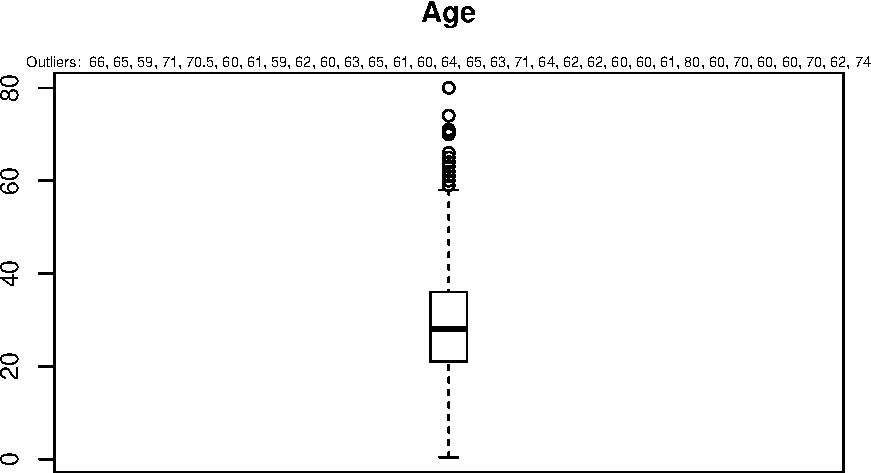
\includegraphics{titanic_data_analysis_PRA2_files/figure-latex/unnamed-chunk-11-1.pdf}

\begin{Shaded}
\begin{Highlighting}[]
\NormalTok{train_df <-}\StringTok{ }\NormalTok{train_df[}\OperatorTok{-}\KeywordTok{which}\NormalTok{(train_df}\OperatorTok{$}\NormalTok{Age }\OperatorTok\StringTok{ }\NormalTok{outlier_values),] }\CommentTok{# los eliminamos}
\end{Highlighting}
\end{Shaded}

Los valores extremos se sitúan a partir de los 66 años en adelante.

\begin{Shaded}
\begin{Highlighting}[]
\KeywordTok{library}\NormalTok{(ggplot2)}
\KeywordTok{ggplot}\NormalTok{(train_df, }\KeywordTok{aes}\NormalTok{(}\DataTypeTok{x =}\NormalTok{ Age)) }\OperatorTok{+}\StringTok{ }\KeywordTok{geom_histogram}\NormalTok{(}\KeywordTok{aes}\NormalTok{(}\DataTypeTok{y =}\NormalTok{ ..density..), }\DataTypeTok{binwidth=}\DecValTok{2}\NormalTok{, }\DataTypeTok{color=}\StringTok{'blue'}\NormalTok{, }\DataTypeTok{fill=}\StringTok{"white"}\NormalTok{) }\OperatorTok{+}\StringTok{ }\KeywordTok{geom_density}\NormalTok{(}\DataTypeTok{color=}\StringTok{'red'}\NormalTok{)}
\end{Highlighting}
\end{Shaded}

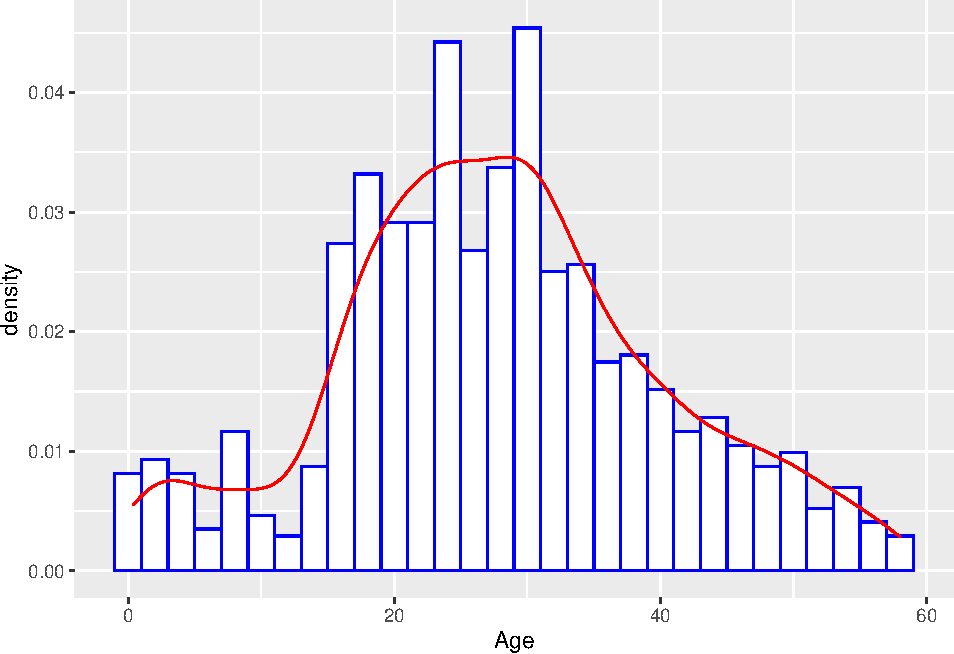
\includegraphics{titanic_data_analysis_PRA2_files/figure-latex/unnamed-chunk-12-1.pdf}

Observamos en el histograma superior que la distribución parece ser
gaussiana.

\begin{Shaded}
\begin{Highlighting}[]
\NormalTok{outlier_values <-}\StringTok{ }\KeywordTok{boxplot.stats}\NormalTok{(train_df}\OperatorTok{$}\NormalTok{Fare)}\OperatorTok{$}\NormalTok{out}
\KeywordTok{boxplot}\NormalTok{(train_df}\OperatorTok{$}\NormalTok{Fare, }\DataTypeTok{main=}\StringTok{"Fare"}\NormalTok{, }\DataTypeTok{boxwex=}\FloatTok{0.1}\NormalTok{)}
\KeywordTok{mtext}\NormalTok{(}\KeywordTok{paste}\NormalTok{(}\StringTok{"Outliers: "}\NormalTok{, }\KeywordTok{paste}\NormalTok{(outlier_values, }\DataTypeTok{collapse=}\StringTok{", "}\NormalTok{)), }\DataTypeTok{cex=}\FloatTok{0.6}\NormalTok{)}
\end{Highlighting}
\end{Shaded}

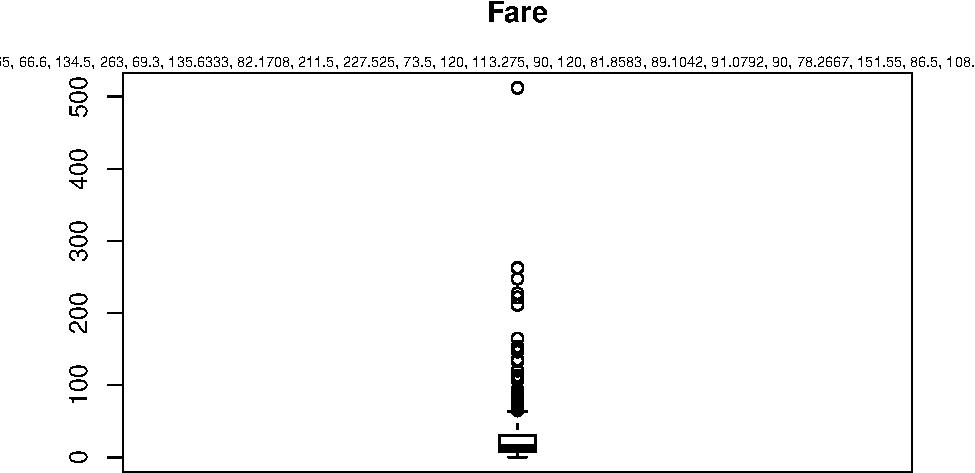
\includegraphics{titanic_data_analysis_PRA2_files/figure-latex/unnamed-chunk-13-1.pdf}

\begin{Shaded}
\begin{Highlighting}[]
\NormalTok{train_df <-}\StringTok{ }\NormalTok{train_df[}\OperatorTok{-}\KeywordTok{which}\NormalTok{(train_df}\OperatorTok{$}\NormalTok{Fare }\OperatorTok\StringTok{ }\NormalTok{outlier_values),] }\CommentTok{# los eliminamos}
\end{Highlighting}
\end{Shaded}

Por lo visto, era extraño que el ticket superara el coste de los 70
dolares. Los costes más altos se deberían o bien a errores o bien a
Cabinas con unas condiciones privilegiadas. Y por lo visto, no era raro
pasar gratis, ya que el cero lo considera un valor común más.

\begin{Shaded}
\begin{Highlighting}[]
\KeywordTok{ggplot}\NormalTok{(train_df, }\KeywordTok{aes}\NormalTok{(}\DataTypeTok{x =}\NormalTok{ Fare)) }\OperatorTok{+}\StringTok{ }\KeywordTok{geom_histogram}\NormalTok{(}\KeywordTok{aes}\NormalTok{(}\DataTypeTok{y =}\NormalTok{ ..density..), }\DataTypeTok{binwidth=}\DecValTok{2}\NormalTok{, }\DataTypeTok{color=}\StringTok{'blue'}\NormalTok{, }\DataTypeTok{fill=}\StringTok{"white"}\NormalTok{) }\OperatorTok{+}\StringTok{ }\KeywordTok{geom_density}\NormalTok{(}\DataTypeTok{color=}\StringTok{'red'}\NormalTok{)}
\end{Highlighting}
\end{Shaded}

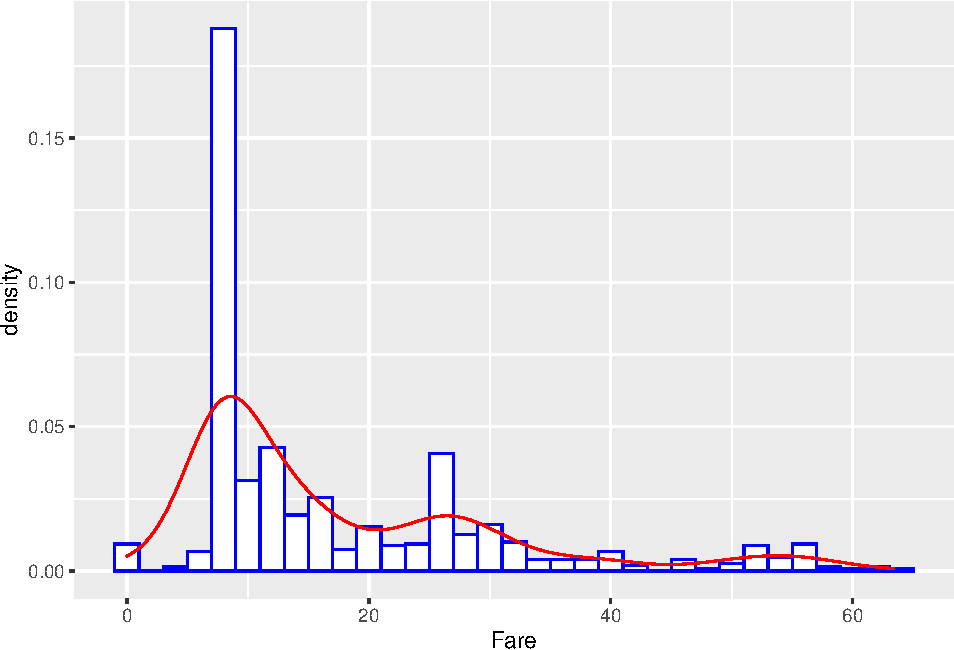
\includegraphics{titanic_data_analysis_PRA2_files/figure-latex/unnamed-chunk-14-1.pdf}

\hypertarget{anuxe1lisis-de-los-datos.}{%
\subsubsection{4. Análisis de los
datos.}\label{anuxe1lisis-de-los-datos.}}

\textbf{4.1. Selección de los grupos de datos que se quieren
analizar/comparar (planificación de los análisis a aplicar).}

El nombre es prescindible puesto que ya tenemos un identificador ya. Aun
así, podrían llegar a deducirse información útil como la nacionalidad
(aproximada) del pasajero. Pero esta tarea no aplica al alcance de esta
tarea.

\begin{Shaded}
\begin{Highlighting}[]
\NormalTok{train_df}\OperatorTok{$}\NormalTok{Name <-}\StringTok{ }\OtherTok{NULL}
\end{Highlighting}
\end{Shaded}

Del mismo modo, podríamos asumir que el ticket se trata del
identificador del tripulante y que no contiene otro tipo de información
deducible o complementaria, más allá del orden de compra del ticket, lo
cual, dificilmente interviene en la supervivencia del pasajero. Además,
ya tenemos un ID por lo que prescindiremos del atributo.

\begin{Shaded}
\begin{Highlighting}[]
\NormalTok{train_df}\OperatorTok{$}\NormalTok{Ticket <-}\StringTok{ }\OtherTok{NULL}
\end{Highlighting}
\end{Shaded}

\textbf{4.2. Comprobación de la normalidad y homogeneidad de la
varianza.}

Veamos si los atributos numéricos Age y Fare siguen una distribución
normal.

Para ambos casos y según el teorema del límite central, al ser el
tamaños de la muestras suficientemente grande (\textgreater{} 30),
siguen \textbf{distirbución normal estándar}.

Ahora aplicaremos el \textbf{test de Shapiro} para confirmar esta
distribución:

\begin{Shaded}
\begin{Highlighting}[]
\NormalTok{alpha =}\StringTok{ }\FloatTok{0.05}
\KeywordTok{shapiro.test}\NormalTok{(train_df}\OperatorTok{$}\NormalTok{Age)}\OperatorTok{$}\NormalTok{p.value }\OperatorTok{>}\StringTok{ }\NormalTok{alpha}
\end{Highlighting}
\end{Shaded}

\begin{verbatim}
## [1] FALSE
\end{verbatim}

Age tiene una distribución normal.

\begin{Shaded}
\begin{Highlighting}[]
\NormalTok{alpha =}\StringTok{ }\FloatTok{0.05}
\KeywordTok{shapiro.test}\NormalTok{(train_df}\OperatorTok{$}\NormalTok{Fare)}\OperatorTok{$}\NormalTok{p.value }\OperatorTok{>}\StringTok{ }\NormalTok{alpha}
\end{Highlighting}
\end{Shaded}

\begin{verbatim}
## [1] FALSE
\end{verbatim}

Fare tiene una distribución normal.

Ambos atributos pasan el test al ser los valores de p superiores al del
nivel de significacia 0.05.

Por otro lado, utilizamos el gráfico Q-Q, para diagnosticar la
desviación de los datos de la muestra en relación con una población
normal:

\begin{Shaded}
\begin{Highlighting}[]
\KeywordTok{qqnorm}\NormalTok{(train_df}\OperatorTok{$}\NormalTok{Age)}
\KeywordTok{qqline}\NormalTok{(train_df}\OperatorTok{$}\NormalTok{Age)}
\end{Highlighting}
\end{Shaded}

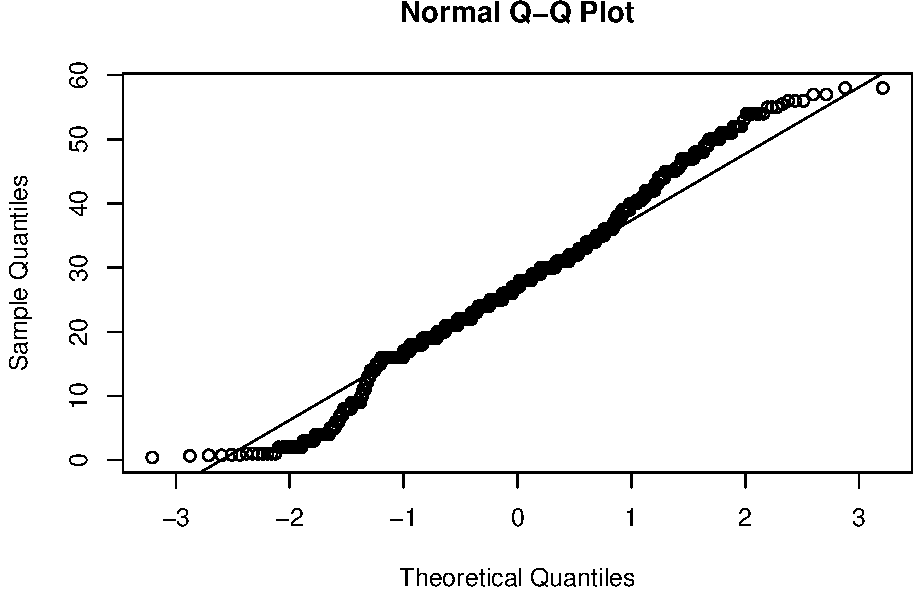
\includegraphics{titanic_data_analysis_PRA2_files/figure-latex/unnamed-chunk-19-1.pdf}

\begin{Shaded}
\begin{Highlighting}[]
\KeywordTok{qqnorm}\NormalTok{(train_df}\OperatorTok{$}\NormalTok{Fare)}
\KeywordTok{qqline}\NormalTok{(train_df}\OperatorTok{$}\NormalTok{Fare)}
\end{Highlighting}
\end{Shaded}

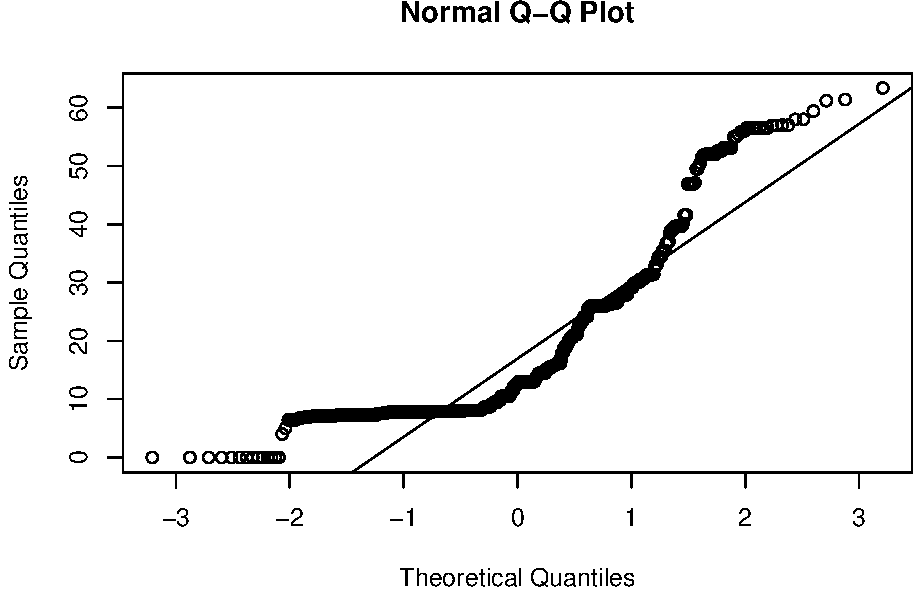
\includegraphics{titanic_data_analysis_PRA2_files/figure-latex/unnamed-chunk-20-1.pdf}

Ambos conjuntos de datos cumplen la linealidad de la diagonal
(aproximadamente), confirmando el resultado del test Shapiro-Wilk y con
ello la normalidad de sus distribuciones.

\textbf{4.3. Aplicación de pruebas estadísticas para comparar los grupos
de datos. En función de los datos y el objetivo del estudio, aplicar
pruebas de contraste de hipótesis, correlaciones, regresiones, etc.
Aplicar al menos tres métodos de análisis diferentes.}

\textbf{Correlaciones:}

\textbf{Contraste de hipótesis:}

\begin{itemize}
\item
  \textbf{Hipótesis nula o de partida unilateral (H0):} el coste medio
  de los tickets de los supervivientes supera en 6 dolares al coste de
  los que no sobrevivieron.
\item
  \textbf{Hipótesis alternativa (H1):} el coste medio de los tickets de
  los supervivientes es igual o menor a 6 dolares al coste de los que no
  sobrevivieron.
\end{itemize}

Confirmamos distribuciones normales de los subconjuntos poblacionales
(t-student al ser muestrales).

\begin{Shaded}
\begin{Highlighting}[]
\NormalTok{alpha =}\StringTok{ }\FloatTok{0.05}
\KeywordTok{shapiro.test}\NormalTok{(train_df}\OperatorTok{$}\NormalTok{Fare[ train_df}\OperatorTok{$}\NormalTok{Survived}\OperatorTok{==}\DecValTok{1}\NormalTok{ ])}\OperatorTok{$}\NormalTok{p.value }\OperatorTok{>}\StringTok{ }\NormalTok{alpha}
\end{Highlighting}
\end{Shaded}

\begin{verbatim}
## [1] FALSE
\end{verbatim}

\begin{Shaded}
\begin{Highlighting}[]
\NormalTok{alpha =}\StringTok{ }\FloatTok{0.05}
\KeywordTok{shapiro.test}\NormalTok{(train_df}\OperatorTok{$}\NormalTok{Fare[ train_df}\OperatorTok{$}\NormalTok{Survived}\OperatorTok{==}\DecValTok{0}\NormalTok{ ])}\OperatorTok{$}\NormalTok{p.value }\OperatorTok{>}\StringTok{ }\NormalTok{alpha}
\end{Highlighting}
\end{Shaded}

\begin{verbatim}
## [1] FALSE
\end{verbatim}

Efectivamente, lo son. Por tanto:

\begin{Shaded}
\begin{Highlighting}[]
\KeywordTok{t.test}\NormalTok{(train_df}\OperatorTok{$}\NormalTok{Fare[ train_df}\OperatorTok{$}\NormalTok{Survived}\OperatorTok{==}\DecValTok{1}\NormalTok{ ], train_df}\OperatorTok{$}\NormalTok{Fare[ train_df}\OperatorTok{$}\NormalTok{Survived}\OperatorTok{==}\DecValTok{0}\NormalTok{ ],}\DataTypeTok{alternative=}\StringTok{"greater"}\NormalTok{, }\DataTypeTok{var.equal=}\OtherTok{FALSE}\NormalTok{)}
\end{Highlighting}
\end{Shaded}

\begin{verbatim}
## 
##  Welch Two Sample t-test
## 
## data:  train_df$Fare[train_df$Survived == 1] and train_df$Fare[train_df$Survived == 0]
## t = 6.4296, df = 428.7, p-value = 1.709e-10
## alternative hypothesis: true difference in means is greater than 0
## 95 percent confidence interval:
##  5.095916      Inf
## sample estimates:
## mean of x mean of y 
##  21.99375  15.14090
\end{verbatim}

Se apoya la hipótesis nula de que las tarifas de los supervivientes
superaban los 6 dolares a las de los no supervivientes con una tasa de
acierto del 95\%.

\textbf{Regresión logística:}

Al ser la etiqueta supervisada binaria, aplicamos una regresión
logística:

\begin{Shaded}
\begin{Highlighting}[]
\NormalTok{glm.fit <-}\StringTok{ }\KeywordTok{lm}\NormalTok{(}\KeywordTok{as.numeric}\NormalTok{(Survived) }\OperatorTok{~}\StringTok{ }\NormalTok{Pclass }\OperatorTok{+}\StringTok{ }\NormalTok{Sex }\OperatorTok{+}\StringTok{ }\NormalTok{Age }\OperatorTok{+}\StringTok{ }\NormalTok{SibSp }\OperatorTok{+}\StringTok{ }\NormalTok{Parch }\OperatorTok{+}\StringTok{ }\NormalTok{Fare }\OperatorTok{+}\StringTok{ }\NormalTok{Cabin }\OperatorTok{+}\StringTok{ }\NormalTok{Embarked, }\DataTypeTok{data =}\NormalTok{ train_df)}
\KeywordTok{summary}\NormalTok{(glm.fit)}
\end{Highlighting}
\end{Shaded}

\begin{verbatim}
## 
## Call:
## lm(formula = as.numeric(Survived) ~ Pclass + Sex + Age + SibSp + 
##     Parch + Fare + Cabin + Embarked, data = train_df)
## 
## Residuals:
##      Min       1Q   Median       3Q      Max 
## -0.81570 -0.16736 -0.06338  0.16424  1.06002 
## 
## Coefficients:
##                   Estimate Std. Error t value Pr(>|t|)    
## (Intercept)       1.549287   0.383652   4.038 6.03e-05 ***
## Pclass2          -0.070008   0.102400  -0.684  0.49443    
## Pclass3          -0.212683   0.104888  -2.028  0.04300 *  
## Sexmale          -0.456888   0.033951 -13.457  < 2e-16 ***
## Age              -0.008619   0.001543  -5.585 3.45e-08 ***
## SibSp1           -0.047497   0.042155  -1.127  0.26028    
## SibSp2           -0.115644   0.092222  -1.254  0.21030    
## SibSp3           -0.524838   0.113775  -4.613 4.79e-06 ***
## SibSp4           -0.424583   0.107691  -3.943 8.94e-05 ***
## SibSp5           -0.534149   0.189049  -2.825  0.00487 ** 
## Parch1            0.062410   0.054702   1.141  0.25432    
## Parch2           -0.008139   0.069335  -0.117  0.90659    
## Parch3            0.084197   0.170547   0.494  0.62169    
## Parch4           -0.368687   0.218321  -1.689  0.09175 .  
## Parch5           -0.273988   0.174505  -1.570  0.11688    
## Parch6           -0.577587   0.379307  -1.523  0.12831    
## Fare              0.005430   0.002080   2.611  0.00925 ** 
## CabinA14          0.128996   0.525890   0.245  0.80631    
## CabinA16          0.696892   0.526046   1.325  0.18571    
## CabinA19          0.188304   0.525720   0.358  0.72032    
## CabinA20          1.068294   0.525315   2.034  0.04240 *  
## CabinA24         -0.069699   0.525458  -0.133  0.89452    
## CabinA26          1.197502   0.523983   2.285  0.02261 *  
## CabinA31          1.084030   0.523349   2.071  0.03872 *  
## CabinA32          0.070902   0.525326   0.135  0.89268    
## CabinA36          0.273471   0.531359   0.515  0.60696    
## CabinA6           0.985877   0.525184   1.877  0.06094 .  
## CabinA7           0.223591   0.524289   0.426  0.66991    
## CabinB102         0.221755   0.531388   0.417  0.67659    
## CabinB18          0.332029   0.457499   0.726  0.46826    
## CabinB20          0.653697   0.458225   1.427  0.15418    
## CabinB37          0.246238   0.524573   0.469  0.63894    
## CabinB38          0.181008   0.525643   0.344  0.73069    
## CabinB39          0.379669   0.527222   0.720  0.47170    
## CabinB4           0.679427   0.524985   1.294  0.19606    
## CabinB42          0.481282   0.527111   0.913  0.36155    
## CabinB50          1.017791   0.523367   1.945  0.05224 .  
## CabinB51 B53 B55  0.194602   0.529868   0.367  0.71354    
## CabinB71         -0.030371   0.526756  -0.058  0.95404    
## CabinB94          0.282090   0.531370   0.531  0.59569    
## CabinC101         0.773341   0.534591   1.447  0.14849    
## CabinC103         0.836171   0.527821   1.584  0.11364    
## CabinC104         1.219893   0.525565   2.321  0.02059 *  
## CabinC106         1.159558   0.525263   2.208  0.02762 *  
## CabinC110         0.060042   0.525503   0.114  0.90907    
## CabinC111         0.015486   0.523652   0.030  0.97642    
## CabinC118         0.002821   0.526753   0.005  0.99573    
## CabinC123         0.278308   0.457377   0.608  0.54308    
## CabinC124         0.186487   0.455915   0.409  0.68265    
## CabinC126         0.848927   0.457375   1.856  0.06390 .  
## CabinC128         0.139430   0.525001   0.266  0.79065    
## CabinC148         0.968790   0.523581   1.850  0.06472 .  
## CabinC30          0.245751   0.525763   0.467  0.64036    
## CabinC47          1.022135   0.523432   1.953  0.05128 .  
## CabinC49         -0.274242   0.525269  -0.522  0.60178    
## CabinC52          1.036036   0.455583   2.274  0.02329 *  
## CabinC90          0.388747   0.524626   0.741  0.45896    
## CabinD            0.550732   0.437690   1.258  0.20875    
## CabinD10 D12      0.699371   0.527045   1.327  0.18499    
## CabinD17          0.757659   0.457747   1.655  0.09837 .  
## CabinD19          1.061432   0.526640   2.015  0.04427 *  
## CabinD21          0.547965   0.527500   1.039  0.29929    
## CabinD28          0.341968   0.529167   0.646  0.51835    
## CabinD30         -0.139776   0.527599  -0.265  0.79115    
## CabinD35          0.770578   0.459176   1.678  0.09380 .  
## CabinD45          1.136415   0.525242   2.164  0.03086 *  
## CabinD46          0.157677   0.525095   0.300  0.76406    
## CabinD47          0.509604   0.531817   0.958  0.33830    
## CabinD56          1.229786   0.532014   2.312  0.02111 *  
## CabinD6           0.024364   0.525446   0.046  0.96303    
## CabinE10          1.382103   0.531671   2.600  0.00955 ** 
## CabinE101         0.719431   0.439005   1.639  0.10175    
## CabinE12          1.206866   0.525748   2.296  0.02202 *  
## CabinE121         0.933619   0.466091   2.003  0.04558 *  
## CabinE17          1.232724   0.525894   2.344  0.01938 *  
## CabinE24          1.126408   0.455924   2.471  0.01374 *  
## CabinE25          1.104588   0.455936   2.423  0.01568 *  
## CabinE31          0.049095   0.527450   0.093  0.92587    
## CabinE33          0.308968   0.460044   0.672  0.50207    
## CabinE36          0.400141   0.525229   0.762  0.44643    
## CabinE44          0.336367   0.457674   0.735  0.46264    
## CabinE46          0.121124   0.525812   0.230  0.81789    
## CabinE50          0.869508   0.525093   1.656  0.09822 .  
## CabinE58          0.203473   0.525821   0.387  0.69891    
## CabinE63          0.133353   0.524948   0.254  0.79955    
## CabinE77         -0.015281   0.534768  -0.029  0.97721    
## CabinE8           0.726592   0.457540   1.588  0.11276    
## CabinF E69        0.647737   0.533654   1.214  0.22527    
## CabinF G63        0.470468   0.532160   0.884  0.37698    
## CabinF G73        0.298082   0.462943   0.644  0.51988    
## CabinF2           0.644804   0.440117   1.465  0.14339    
## CabinF33          0.738852   0.439172   1.682  0.09298 .  
## CabinF38          0.305347   0.532864   0.573  0.56682    
## CabinF4           0.641875   0.473564   1.355  0.17576    
## CabinG6           0.225469   0.427735   0.527  0.59829    
## CabinSin cabina   0.434138   0.380963   1.140  0.25488    
## CabinT            0.132405   0.524967   0.252  0.80095    
## EmbarkedQ         0.040051   0.061174   0.655  0.51289    
## EmbarkedS        -0.029716   0.044404  -0.669  0.50360    
## ---
## Signif. codes:  0 '***' 0.001 '**' 0.01 '*' 0.05 '.' 0.1 ' ' 1
## 
## Residual standard error: 0.3698 on 648 degrees of freedom
## Multiple R-squared:  0.4753, Adjusted R-squared:  0.396 
## F-statistic: 5.991 on 98 and 648 DF,  p-value: < 2.2e-16
\end{verbatim}

Los atributos que más impacto tienen en el resultado de la supervivencia
del naufragio son:

\begin{itemize}
\item
  Sexmale: Los hombres tenían una probabilidad muy alta de no
  sobrevivir, probablemente porque fueron los últimos en entrar a los
  botes salvavidas, priorizando a mujeres y niños.
\item
  Age: Cuanto mayor eras, menos probabilidades de supervivencia tenías,
  muy probablemente, por la misma razón que la anteriormente explicada.
\item
  SibSp3, SibSp4, SibSp5: tener muchos familiares a bordo no era una
  garantía de supervivencia, probablemente, por tener que priorizarles o
  perder tiempo velando por su supervivencia durante el naufragio.
\item
  Fare: Haber pagado una tarifa alta contribuía en cierta medida a la
  supervivencia, probablemente vinculado a la relevancia de esas
  personas y/o a su prioridad en botes salvavidas, incluida en las
  condiciones de embarque.
\item
  CabinA20, CabinA26, CabinA31 Algunas cabinas fueron afortunadas,
  lógicamente por su ubicación, pudieron, quizás, llegar antes a los
  botes salvavidas.
\end{itemize}

\textbf{5. Representación de los resultados a partir de tablas y
gráficas.}

Relación entre el género y la supervivencia:

\begin{Shaded}
\begin{Highlighting}[]
\KeywordTok{ggplot}\NormalTok{(train_df, }\KeywordTok{aes}\NormalTok{(Sex, ..count..)) }\OperatorTok{+}\StringTok{ }\KeywordTok{geom_bar}\NormalTok{(}\KeywordTok{aes}\NormalTok{(}\DataTypeTok{fill =}\NormalTok{ Survived), }\DataTypeTok{position =} \StringTok{"dodge"}\NormalTok{)}
\end{Highlighting}
\end{Shaded}

\includegraphics{titanic_data_analysis_PRA2_files/figure-latex/unnamed-chunk-25-1.pdf}

Confirmamos que ser hombres perjudicaba a la supervivencia.

Relación entre el parenteso ``horizontal'' y la supervivencia:

\begin{Shaded}
\begin{Highlighting}[]
\KeywordTok{ggplot}\NormalTok{(train_df, }\KeywordTok{aes}\NormalTok{(SibSp, ..count..)) }\OperatorTok{+}\StringTok{ }\KeywordTok{geom_bar}\NormalTok{(}\KeywordTok{aes}\NormalTok{(}\DataTypeTok{fill =}\NormalTok{ Survived), }\DataTypeTok{position =} \StringTok{"dodge"}\NormalTok{)}
\end{Highlighting}
\end{Shaded}

\includegraphics{titanic_data_analysis_PRA2_files/figure-latex/unnamed-chunk-26-1.pdf}

Confirmamos que a mayor número de familiares, menor probabilidad de
supervivencia.

Relación entre la edad y la supervivencia:

\begin{Shaded}
\begin{Highlighting}[]
\KeywordTok{boxplot}\NormalTok{(Age}\OperatorTok{~}\NormalTok{Survived,}
\DataTypeTok{data=}\NormalTok{train_df,}
\DataTypeTok{xlab=}\StringTok{"Survived"}\NormalTok{,}
\DataTypeTok{ylab=}\StringTok{"Age"}\NormalTok{,}
\DataTypeTok{col=}\StringTok{"orange"}\NormalTok{,}
\DataTypeTok{border=}\StringTok{"brown"}
\NormalTok{)}
\end{Highlighting}
\end{Shaded}

\includegraphics{titanic_data_analysis_PRA2_files/figure-latex/unnamed-chunk-27-1.pdf}

Confirmamos que los que sobrevivieron eran algo más jóvenes que los que
no, sobre los 25 años de media.

Relación entre la tarifa y la supervivencia:

\begin{Shaded}
\begin{Highlighting}[]
\KeywordTok{boxplot}\NormalTok{(Fare}\OperatorTok{~}\NormalTok{Survived,}
\DataTypeTok{data=}\NormalTok{train_df,}
\DataTypeTok{xlab=}\StringTok{"Survived"}\NormalTok{,}
\DataTypeTok{ylab=}\StringTok{"Fare"}\NormalTok{,}
\DataTypeTok{col=}\StringTok{"orange"}\NormalTok{,}
\DataTypeTok{border=}\StringTok{"brown"}
\NormalTok{)}
\end{Highlighting}
\end{Shaded}

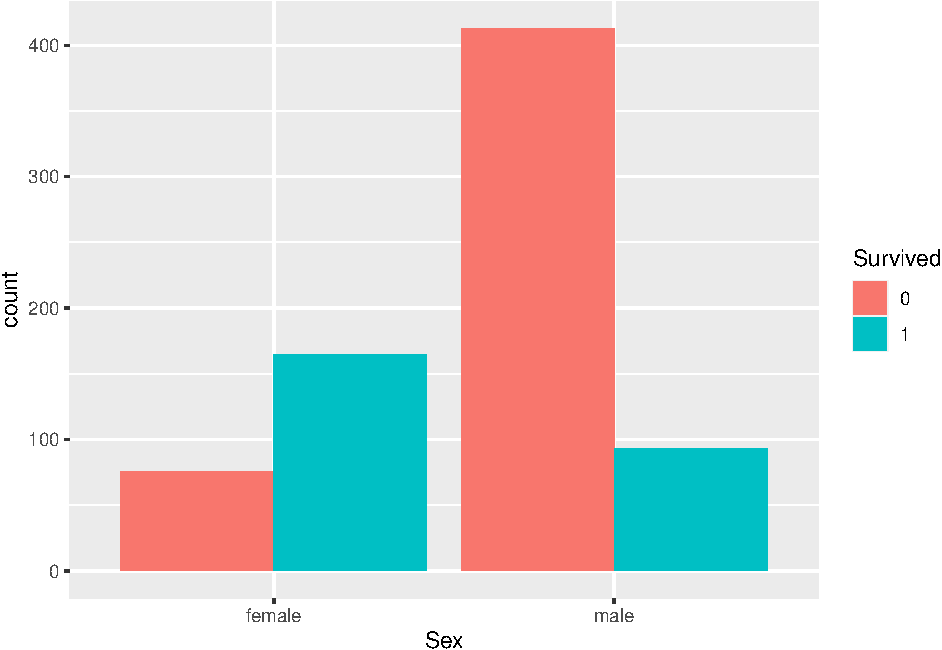
\includegraphics{titanic_data_analysis_PRA2_files/figure-latex/unnamed-chunk-28-1.pdf}

Confirmamos que los que sobrevivieron también tenían tarifas más caras.

\end{document}
